

\newcommand{\mriinput}[2]{
    \def\mridepth{3}
    \node[yslant=1, inner sep=0pt] (input) at (#1, #2) {
        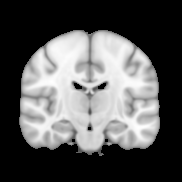
\includegraphics[width=5cm, height=8.5cm]{data/mri.png}
    };
    \draw[fill=black] (input.north east) --
        ($ (input.north east) - (\mridepth, 0) $) --
        ($ (input.north west) - (\mridepth, 0) $) --
        (input.north west) -- cycle;
    \draw[fill=black] (input.north west) --
        ($ (input.north west) - (\mridepth, 0) $) --
        ($ (input.south west) - (\mridepth, 0) $) --
        (input.south west) -- cycle;
    \draw[] (input.north east) --
        ($ (input.north east) + (\mridepth, 0) $) --
        ($ (input.north west) + (\mridepth, 0) $) --
        (input.north west) -- cycle;
    \draw[]  ($ (input.north west) + (\mridepth, 0) $) --
        ($ (input.south west) + (\mridepth, 0) $) --
        (input.south west);
    \draw[] ($ (input.north east) + (\mridepth, 0) $) --
        ($ (input.south east) + (\mridepth, 0) $) --
        ($ (input.south west) + (\mridepth, 0) $);
    \node[
        anchor=south,
        align=center,
        font=\fontsize{32}{32}\linespread{0.8}\selectfont,
        text depth=0
    ] at ($ (input.north east) + (0, 0.2) $) {
        \textit{Structural MRI}
    };
}

\newcommand{\convside}[6]{
    \node[
        fill=#5,
        inner sep=0pt,
        outer sep=0pt,
        minimum width=#3,
        minimum height=#4,
        draw=black
    ] (#6) at (#1, #2) {};
}

\newcommand{\convtop}[4]{
    \draw[fill=#4,draw=black] #1 --
    ($ #1 + (#3, #3) $) --
    ($ #1 + (#3+#2, #3) $) --
    ($ #1 + (#2, 0) $);
}

\newcommand{\convfront}[3]{
    \draw[black, fill=#3] #1 --
                        ($ #1 + (1*#2, 1*#2) $) --
                        ($ #1 + (1*#2, 1*#2 - 2*#2) $) --
                        ($ #1 + (0, -2*#2) $);
}


\newcommand{\convchannel}[5]{
    \def\huemin{20}
    \def\huemax{80}
    \pgfmathsetmacro{\iterations}{#5-1}
    \foreach \i in {0,...,\iterations} {
        \pgfmathsetmacro{\hue}{int(random(\huemin, \huemax))}
        \convside{#1}{#2+\i*-0.75}{#3}{#4/#5}{blue!\hue}{n\i0}

        \foreach \j in {0,...,\iterations} {
            \pgfmathsetmacro{\innerhue}{int(random(\huemin, \huemax))}
            \ifnum\j=0
                \pgfmathsetmacro{\innerhue}{\hue}
            \fi
            \convfront{($ (n00.north east) + (0.5*\j*#4/#5, 0.5*\j*#4/#5 - \i*#4/#5) $)}{0.5*#4/#5}{blue!\innerhue}

            \ifnum\i=0
                \convtop{($ (n\i0.north west) + (0.5*\j*#4/#5, 0.5*\j*#4/#5) $)}{#3}{0.5*#4/#5}{blue!\innerhue}
            \fi
        }
    }
}

\newcommand{\convlayer}[6]{
    \pgfmathsetmacro{\iterations}{#6-1}
    \foreach \i in {0,...,\iterations}{
        \pgfmathsetmacro{\x}{#1 + \i * 0.33}
        \convchannel{\x}{#2}{#3}{#4}{#5}
    }
}

\newcommand{\cnnarrow}[2]{
    \begin{scope}[transparency group, opacity=0.5]
        \draw[-stealth, line width=15pt] #1 -- #2;
    \end{scope}
}

\newcommand{\cnn}[2]{
    \convlayer{#1}{#2-0.25}{0.33cm}{9cm}{12}{3}
    \cnnarrow{(#1 + 3.07, #2 - 2.1)}{(#1+7.5, #2 - 2.1)}
    \convlayer{#1 + 6}{#2-1}{0.33cm}{6cm}{8}{5}%#1 + 6.4
    \cnnarrow{(#1 + 8.97, #2 - 2.1)}{(#1+13, #2 - 2.1)}
    \convlayer{#1 + 11.17}{#2-1.75}{0.33cm}{3cm}{4}{7}%#1 + 11.9
    \cnnarrow{(#1 + 14.07, #2 - 2.1)}{(#1+18, #2 - 2.1)}
    \convlayer{#1 + 15.5}{#2-2.1}{0.33cm}{1.5cm}{2}{9}%#1 + 16.5
    \cnnarrow{(#1 + 18.67, #2 - 2.1)}{(#1+21.06, #2 - 2.1)}

    \draw[thick, dashed] (#1 - 0.67, #2 + 5.125) --
                        (#1 + 19.55, #2 + 5.125) --
                        (#1 + 19.55, #2 - 9.38) --
                        (#1 - 0.67, #2 - 9.38) -- cycle;
    \node[anchor=south, text depth=0, font=\fontsize{32}{32}] at (#1 + 9.95, #2 + 5.3) {
        \textbf{3D Convolutional Neural Network}
    };
}

\newcommand{\lrpchannel}[5]{
    \def\huemin{30}
    \def\huemax{210}
    \colorlet{bgcolor}{black!90}
    \pgfmathsetmacro{\iterations}{#5-1}
    \foreach \i in {0,...,\iterations} {
        \pgfmathsetmacro{\red}{int(random(-150, 100))}
        \colorlet{fillcolor}{bgcolor}

        \ifnum\red>0
            \colorlet{fillcolor}{red!\red!bgcolor}
        \fi

        \convside{#1}{#2+\i*-0.75}{#3}{#4/#5}{fillcolor}{n\i0}

        \foreach \j in {0,...,\iterations} {
            \pgfmathsetmacro{\innerred}{int(random(-150, 100))}
            \colorlet{innerfillcolor}{bgcolor}

            \ifnum\innerred>0
                \colorlet{innerfillcolor}{red!\innerred!bgcolor}
            \fi

            \ifnum\j=0
                \colorlet{innerfillcolor}{fillcolor}
            \fi

            \convfront{($ (n00.north east) + (0.5*\j*#4/#5, 0.5*\j*#4/#5 - \i*#4/#5) $)}{0.5*#4/#5}{innerfillcolor}
            \ifnum\i=0
                \convtop{($ (n\i0.north west) + (0.5*\j*#4/#5, 0.5*\j*#4/#5) $)}{#3}{0.5*#4/#5}{innerfillcolor}
            \fi
        }
    }
}

\newcommand{\lrplayer}[6]{
    \pgfmathsetmacro{\iterations}{#6-1}
    \foreach \i in {0,...,\iterations}{
        \pgfmathsetmacro{\x}{#1 + \i * 0.33}
        \lrpchannel{\x}{#2}{#3}{#4}{#5}
    }
}

\newcommand{\lrp}[2]{

    \lrplayer{#1}{#2-1}{0.33cm}{1.5cm}{2}{9}
    \cnnarrow{(#1 + 3.18, #2 - 1)}{(#1+6, #2 - 1)}
    \lrplayer{#1+4.24}{#2-0.65}{0.33cm}{3cm}{4}{7}
    \cnnarrow{(#1 + 7.14, #2 - 1)}{(#1+13, #2 - 1)}
    \lrplayer{#1 + 8.57}{#2+0.1}{0.33cm}{6cm}{8}{5}
    \cnnarrow{(#1 + 11.55, #2 - 1)}{(#1+15, #2 - 1)}
    \lrplayer{#1 + 13.72}{#2 + 0.85}{0.33cm}{9cm}{12}{3}%#1 + 14.85

    \draw[thick, dashed] (#1 - 0.67, #2 + 6.225) --
                        (#1 + 19.55, #2 + 6.225) --
                        (#1 + 19.55, #2 - 8.275) --
                        (#1 - 0.67, #2 - 8.275) -- cycle;
    \node[anchor=south, text depth=0, font=\fontsize{32}{32}] at (#1 + 9.95, #2 + 6.425) {
        \textbf{Layerwise relevance propagation}
    };
}

\newcommand{\heatmap}[2]{
    \node[yslant=1, inner sep=0pt] (map) at (#1, #2) {
        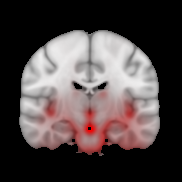
\includegraphics[width=5cm, height=8.5cm]{data/heatmap.png}
    };
    \draw[fill=black] (map.north east) --
        ($ (map.north east) - (\mridepth, 0) $) --
        ($ (map.north west) - (\mridepth, 0) $) --
        (map.north west) -- cycle;
    \draw[fill=black] (map.north west) --
        ($ (map.north west) - (\mridepth, 0) $) --
        ($ (map.south west) - (\mridepth, 0) $) --
        (map.south west) -- cycle;
    \draw[] (map.north east) --
        ($ (map.north east) + (\mridepth, 0) $) --
        ($ (map.north west) + (\mridepth, 0) $) --
        (map.north west) -- cycle;
    \draw[]  ($ (map.north west) + (\mridepth, 0) $) --
        ($ (map.south west) + (\mridepth, 0) $) --
        (map.south west);
    \draw[] ($ (map.north east) + (\mridepth, 0) $) --
        ($ (map.south east) + (\mridepth, 0) $) --
        ($ (map.south west) + (\mridepth, 0) $);
    \node[
        anchor=south,
        align=center,
        font=\fontsize{32}{32}\linespread{0.8}\selectfont,
        text depth=0
    ] at ($ (map.north east) + (0, 0.2) $) {
        \textit{Explanatory}\\
        \textit{heatmap}
    };
}

\newsavebox{\record}
\sbox{\record}{
    \colorlet{cases-default}{red}
    \colorlet{controls-default}{blue}
    \colorlet{healthy-default}{green}
    \colorlet{ninety}{cases-default}
    \colorlet{fifty}{controls-default}
    \colorlet{ten}{healthy-default}

    \newcommand{\mriwidth}{2.59cm}
    \newcommand{\gap}{0.00cm}

    \newcommand{\prediction}[5]{
        \node[circle, inner sep=0pt, outer sep=0pt, minimum size=20pt, draw=#5, fill=#3] (#4) at (\xmin + #1 * \xstep, \ymin+\ymax*#2) {};
    }
    \newcommand{\dashedprediction}[5]{
        \node[circle, inner sep=0pt, outer sep=0pt, minimum size=20pt, draw=#5, fill=#3, dashed, opacity=0.5] (#4) at (\xmin + #1 * \xstep, \ymin+\ymax*#2) {};
    }

    \newcommand{\datenode}[4]{
        \node[
            fill=#3,
            inner sep=0pt,
            anchor=north,
            font=\fontsize{24}{24}\selectfont,
        ] at ($ (\xmin, \ymin) + (#2 * \xstep, -0.2) $) {\textcolor{#4}{#1}};
    }


    \begin{tikzpicture}

        \def\xmin{0}
        \def\ymin{0}
        \def\ystep{0.75}
        \def\ymax{\ystep * 10}
        \def\xstep{2}
        \def\xmax{\xstep * 12}

        \colorlet{faded-black}{black!30}
        \colorlet{faded-white}{white!30}
        \colorlet{faded-cases}{cases-default!30}

        \draw[black] (\xmin, \ymax) -- (\xmax, \ymax) -- (\xmax, \ymin) -- (\xmin, \ymin) -- (\xmin, \ymax);
        \node[anchor=west,font=\fontsize{32}{32}\selectfont] at (\xmax, \ymax) {1.0};
        \node[anchor=west,font=\fontsize{32}{32}\selectfont] at (\xmax, \ymax*0.75) {0.75};
        \node[anchor=west,font=\fontsize{32}{32}\selectfont] at (\xmax, \ymax*0.5) {0.5};
        \node[anchor=west,font=\fontsize{32}{32}\selectfont] at (\xmax, \ymax*0.25) {0.25};
        \node[anchor=west,font=\fontsize{32}{32}\selectfont] at (\xmax, \ymin) {0.0};

        \draw[gray!50, thin] (\xmin, \ymax*0.75) -- (\xmax, \ymax*0.75);
        \draw[gray!50, thin] (\xmin, \ymax*0.5) -- (\xmax, \ymax*0.5);
        \draw[gray!50, thin] (\xmin, \ymax*0.25) -- (\xmax, \ymax*0.25);

        \draw[dashed] (\xmin + 9 * \xstep, \ymin) -- (\xmin + 9 * \xstep, \ymax);
        \draw[dashed] (\xmin + 11 * \xstep, \ymin) -- (\xmin + 11 * \xstep, \ymax);

        \prediction{1}{0.5369713}{blue!40}{p1}{blue!80}
        \prediction{3}{0.5685464}{blue!40}{p2}{blue!80}
        \prediction{5}{0.72608125}{blue!40}{p3}{blue!80}
        \prediction{7}{0.7650767}{blue!40}{p4}{blue!80}
        \prediction{9}{0.78441274}{blue!40}{p5}{blue!80}
        \dashedprediction{11}{0.88}{blue!40}{p6}{blue!80}

        \node[anchor=south, align=center, font=\fontsize{24}{24}\selectfont] at (\xmin + 9 * \xstep, \ymax) {Current\\timepoint};
        \node[anchor=south, align=center, font=\fontsize{24}{24}\selectfont] at (\xmin + 11 * \xstep, \ymax) {Prognostic\\prediction};

        \node[
            anchor=north west,
            fill=black,
            minimum height=1cm,
            minimum width=19.97cm
        ] (fill) at ($ (\xmin - 0.02, \ymin) $) {};
        \node[
            anchor=north west,
            fill=faded-black,
            minimum height=1cm,
            minimum width=4.05cm
        ] (fillgray) at ($ (fill.north east) - (0.00, 0) $) {};
        \node[anchor=north west, inner sep=0pt, outer sep=0pt] (masks) at ($ (fill.south west) + (0.005, 0.009) $) {
            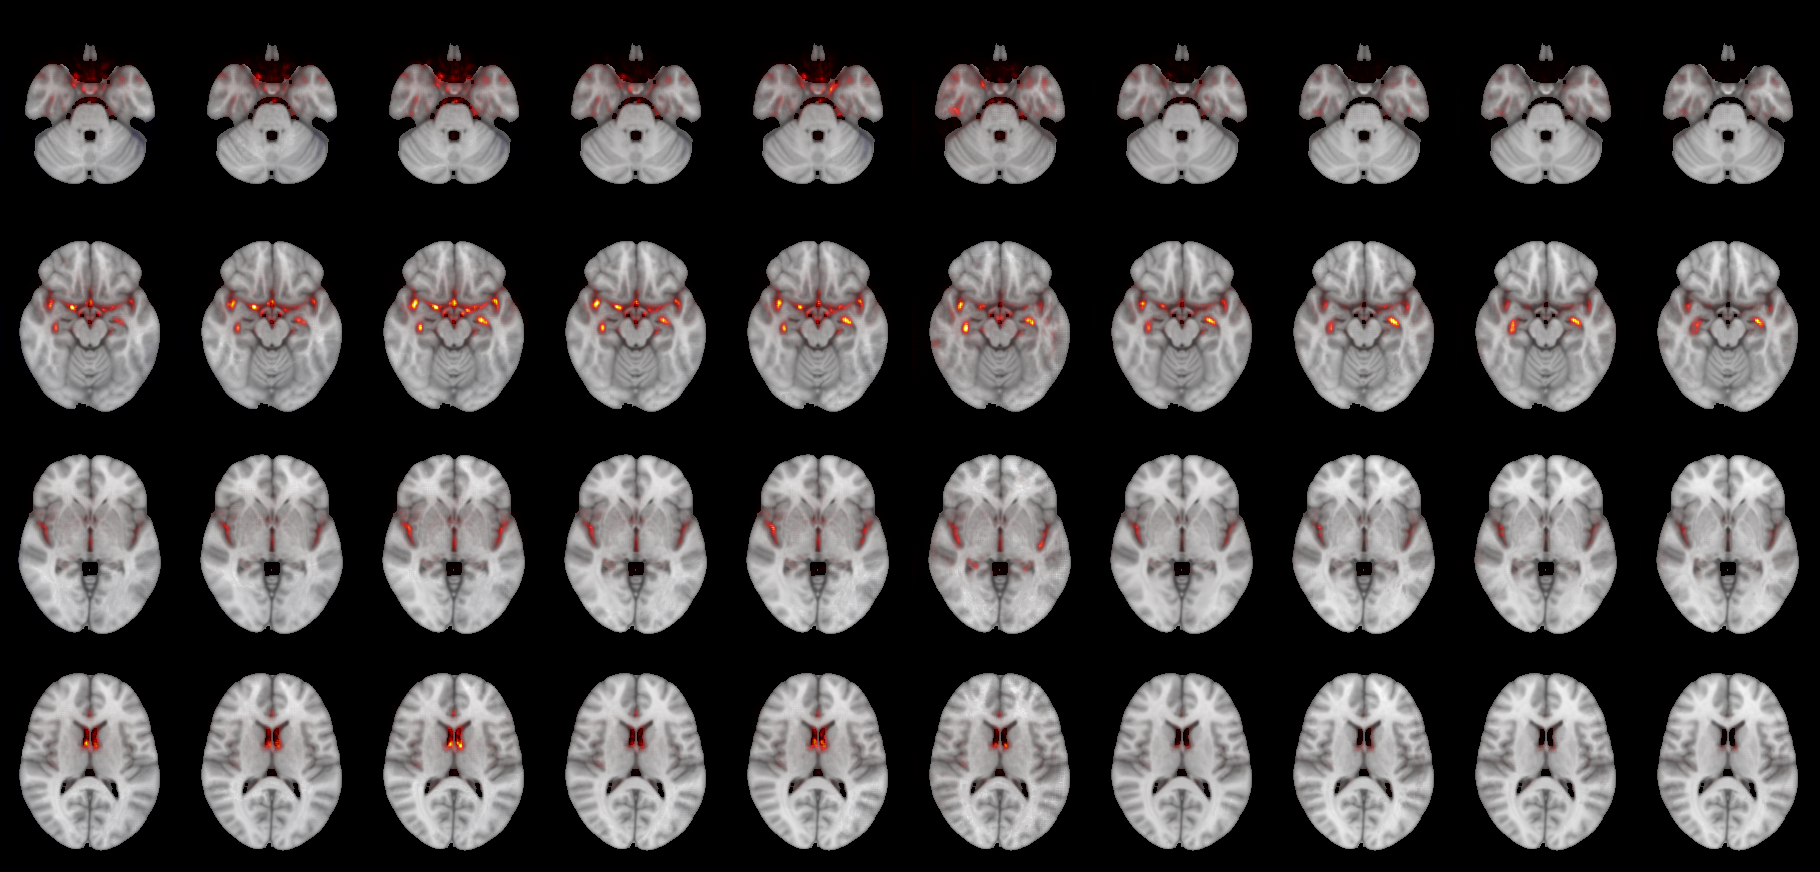
\includegraphics[
                height=4.59cm,
                trim={0cm 15.8cm 32.2cm 7.6cm},
                clip
            ]{data/MCI_to_AD.png}
        };
        \node[anchor=north west, inner sep=0pt, outer sep=0pt] (transparentmasks) at ($ (masks.north east) - (0.02, 0) $) {
            {\transparent{0.3}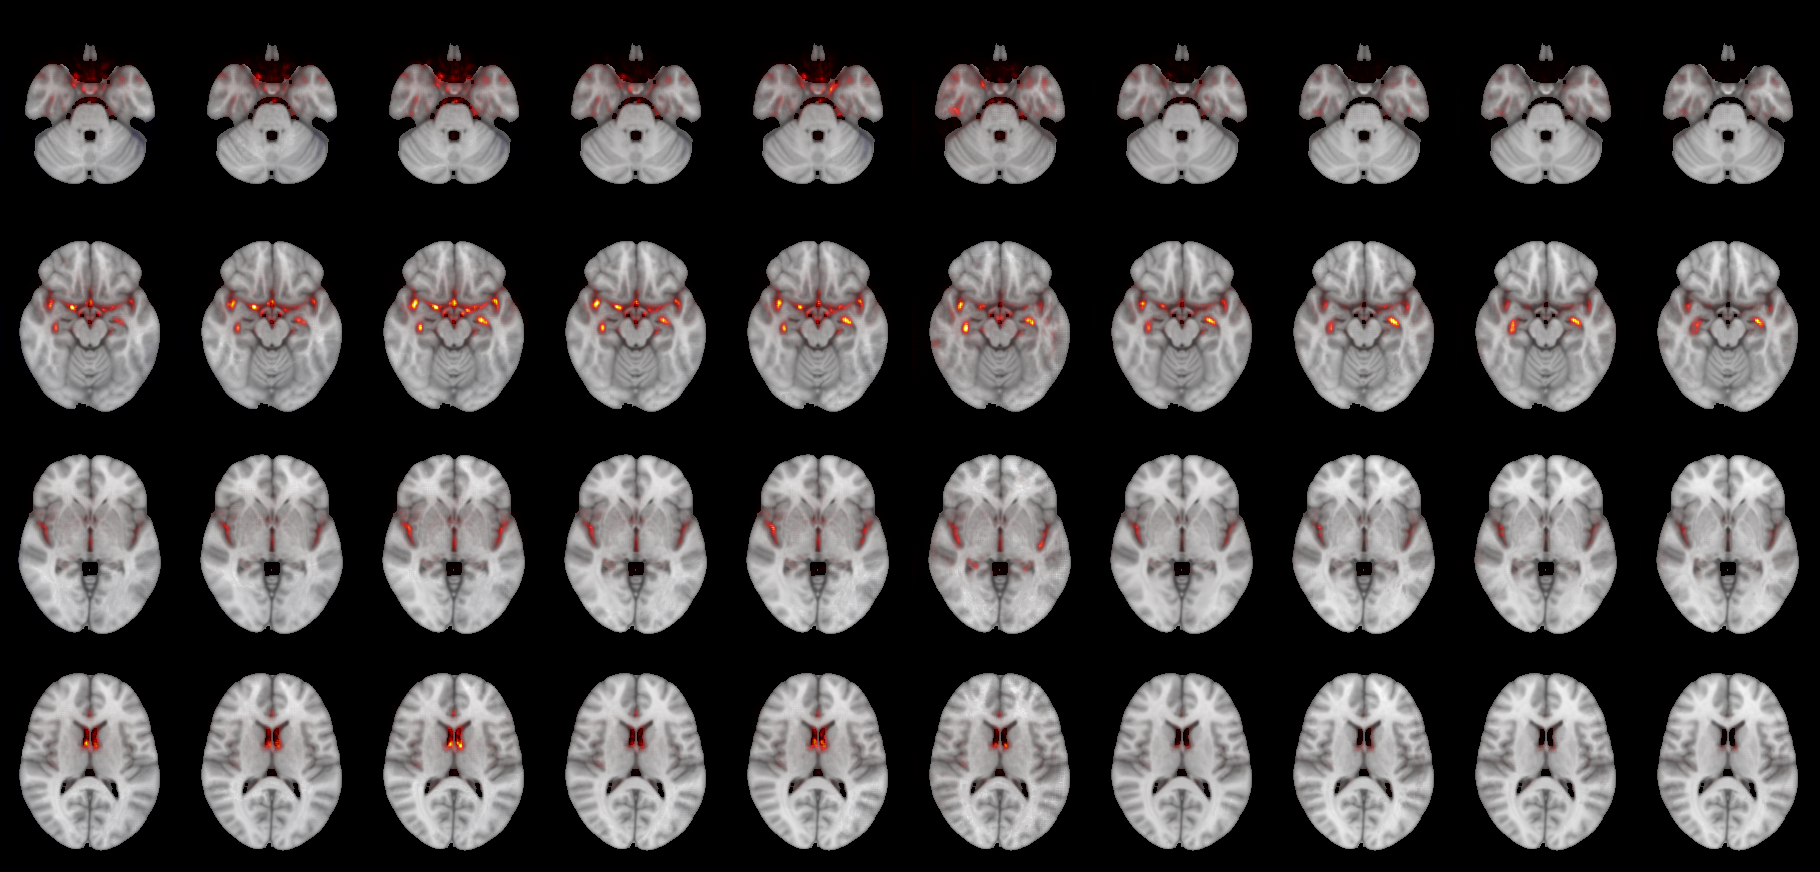
\includegraphics[height=4.59cm, trim={32cm 15.8cm 25.63cm 7.6cm}, clip]{data/MCI_to_AD.png}}
        };

        \datenode{17.07.21}{1}{black}{white}
        \datenode{22.02.22}{3}{black}{white}
        \datenode{05.09.22}{5}{black}{white}
        \datenode{03.04.23}{7}{black}{white}
        \datenode{29.09.23}{9}{black}{white}
        \datenode{13.08.24}{11}{faded-black}{faded-white}

        \node[anchor=south, font=\fontsize{32}{32}\selectfont] at ($ (\xmin + 4.5 * \xstep, \ymax) $) {
            \textbf{Personalized report}
        };
    \end{tikzpicture}
}


\begin{figure}[h]
    \begin{tikzpicture}
        \mriinput{-1.2}{-1.15}

        \cnnarrow{(-1.2, -1.15)}{(7.5, -1.15)}

        \cnn{6}{1}

        \node[align=center,font=\fontsize{32}{32}] (prediction) at (32.55, -1.15) {
            \textit{Predicted probability}\\\textit{of dementia}
        };
        \cnnarrow{(38.05, -1.15)}{(42, -1.15)}

        \lrp{40.23}{-0.15}
        \cnnarrow{(57.02, -1.15)}{(67, -1.15)}

        \heatmap{66.3}{-1.15}

        \node[] (record) at ($ (prediction.south)!0.5!(map.south) - (1, 14) $) {
            \usebox{\record}
        };

        \draw[-stealth, line width=15pt] (prediction.south) to[out=270,in=180, looseness=0.9] ($ (record.west) + (3.23, 1.62)$);
        \draw[-stealth, line width=15pt] ($ (map.south) - (0, 2.51) $) to[out=270,in=0] ($ (record.east) - (3.03, 5) $);

        \node[
            anchor=north west,
            minimum width=36cm,
            minimum height=13.1cm,
            font=\fontsize{24}{28}\selectfont\itshape,
            inner sep=0pt,
            max width=36cm
        ] at ($ (input.south west) - (3, 3.4) $) {
            \textbf{Figure 1: An overview of the proposed analytical pipeline.} A structural T1-weighted magnetic resonance imaging (MRI) scan from a potential patient is given as input to a convolutional neural network (CNN). The CNN, trained to predict whether the scan originates from a patient or a healthy control, computes the probability that the patient has dementia at the current point in time. Next, layerwise relevance propagation is applied to procure a heatmap explaining this prediction, highlighting regions of the brain that contribute towards a predicted diagnosis. When compiled across visits, the predictions and heatmaps can be assembled into a personalized, longitudinal report, encoding trajectories of the absolute quantity, and localization, of dementia-related structural changes in the brain of the patient over time. By analyzing these trajectories, a prognostic prediction can be made about future clinical status. Furthermore, they contains precise information about which brain regions are afflicted, and how this is expected to change. Overall, this pipeline enables personalized diagnostics and prognostics in patients with dementia by providing detailed information about structural, disease-related changes in individual brains.
        };
    \end{tikzpicture}
\end{figure}
